\documentclass{beamer}
\mode<presentation>
{
  \usetheme{Warsaw}
  \definecolor{mcgarnet}{rgb}{0.38, 0, 0.08}
  \definecolor{mcgray}{rgb}{0.6, 0.6, 0.6}
  \setbeamercolor{structure}{fg=mcgarnet,bg=mcgray}
  %\setbeamercovered{transparent}
}


\usepackage[english]{babel}
\usepackage[latin1]{inputenc}
\usepackage{times}
\usepackage[T1]{fontenc}
\usepackage{tikz}
\usepackage{graphicx}

\newcommand{\imagesource}[1]{{\centering\hfill\break\hbox{\scriptsize Image Source:\thinspace{\small\itshape #1}}\par}}

\title{Advanced Magic: Smashing the Stack for Fun and Profit}


\author{Robert Lowe\\}

\institute[Maryville College] % (optional, but mostly needed)
{
  Division of Mathematics and Computer Science\\
  Maryville College
}

\date[]{}
\subject{}

\pgfdeclareimage[height=0.5cm]{university-logo}{images/Maryville-College}
\logo{\pgfuseimage{university-logo}}



\AtBeginSection[]
{
  \begin{frame}<beamer>{Outline}
    \tableofcontents[currentsection]
  \end{frame}
}


\begin{document}

\begin{frame}
  \titlepage
\end{frame}

\begin{frame}{Outline}
  \tableofcontents
\end{frame}


% Structuring a talk is a difficult task and the following structure
% may not be suitable. Here are some rules that apply for this
% solution: 

% - Exactly two or three sections (other than the summary).
% - At *most* three subsections per section.
% - Talk about 30s to 2min per frame. So there should be between about
%   15 and 30 frames, all told.

% - A conference audience is likely to know very little of what you
%   are going to talk about. So *simplify*!
% - In a 20min talk, getting the main ideas across is hard
%   enough. Leave out details, even if it means being less precise than
%   you think necessary.
% - If you omit details that are vital to the proof/implementation,
%   just say so once. Everybody will be happy with that.

\section{Background Knowledge}
\begin{frame}
    \frametitle{Some Notes on Today's Lecture}
    \begin{itemize}[<+->]
        \item A lot of this material comes from "Smashing the Stack for Fun and Profit" by Aleph One (Phrack Issue 49)
        \item Some of this material is dated, as in it can be tricky to make it work.  I have updated examples in the lab to make them functional.
        \item The following only directly works on 32-bit x86 code under Linux, though it is readily adaptable to other platforms.
        \item As is the case with all information, this can be used for good or evil.
        \item Mischief is my aim in teaching you this.
    \end{itemize}
\end{frame}

\begin{frame}[t]
    \frametitle{CPU Registers}
    \begin{columns}[t]
    \column{0.6\textwidth}
    {\bf x86 General Purpose Registers}
    \begin{itemize}[<+->]
        \item {\tt eax} - Accumulator
        \begin{itemize}
            \item {\tt ax} - The lower 16 bits of eax
            \begin{itemize}
                \item {\tt ah} - Upper 8 bits of ax
                \item {\tt al} - Lower 8 bits of ax
            \end{itemize}
        \end{itemize}
        \item {\tt ebx} - Base Register
        \begin{itemize}
            \item {\tt bx}, {\tt bh}, and {\tt bl} as above
        \end{itemize}
        \item {\tt ecx} - Counter Register
        \begin{itemize}
            \item {\tt cx}, {\tt ch}, and {\tt cl} as above
        \end{itemize}
        \item {\tt edx} - Data Register
        \begin{itemize}
            \item {\tt dx}, {\tt dh}, and {\tt dl} as above
        \end{itemize}
    \end{itemize}
    
    \column{0.4\textwidth}
    {\bf x86 Special Registers} 
    \begin{itemize}[<+->]
        \item {\tt eip} - Instruction Pointer
        \item {\tt esi} - Source Index
        \item {\tt edi} - Destination Index
        \item {\tt ebp} - Base Pointer
        \item {\tt esp} - Stack Pointer
    \end{itemize}
    \end{columns}
\end{frame}

\begin{frame}
    \frametitle{Machine Code / Assembly Code}
    \begin{itemize}[<+->]
        \item Machine code is just numbers!
        \item Assembly is the mnemonic representation of those raw numbers.
        \item Example instructions include:
        \begin{itemize}
            \item {\tt movl src, dest}
            \item {\tt jmp addr}
            \item {\tt call addr}
            \item {\tt pushl src}
            \item {\tt popl src}
        \end{itemize}
        \item For a full listing, see the i386 programmer's manual.
        \item Also, look at the gas user's manual for the at\&t syntax!  (it differs from Intel syntax)
    \end{itemize}
\end{frame}

\begin{frame}
    \frametitle{Working in C and Low-Level Exploration}
    \begin{itemize}
        \item We will be using C to better illustrate low-level exploits.
        \item We will be compiling with {\tt gcc -m32} so as to generate 32-bit code (in keeping with our source document)
        \item Using {\tt -S -static} with gcc is a great way to learn assembly.  This will cause the compiler to stop after generating assembly code.
        \item The gdb command {\tt disassemble function} will be used quite frequently as well.
        \item I/O will use {\tt printf} and {\tt gets}, just follow along and you'll get the idea!
        \item Note that while C++ code is generally less susceptible to buffer overflow attacks, you can't rely on that as an absolute.
    \end{itemize}
\end{frame}

\section{Exploring The Stack}
\begin{frame}[fragile]
    \frametitle{What is the Stack?}
    \begin{columns}
    \column{0.6\textwidth}
    \begin{itemize}[<+->]
        \item The stack is just a contiguous block of memory.
        \item The stack grows downwards.  
        \item Each stack "slot" on x86 contains 32-bits.
        \item There are two fundamental operations on a stack:
        \begin{itemize}
            \item {\tt pushl src}
            \item {\tt popl dst}
        \end{itemize}
        \item Pushing decrements {\tt esp} by 4.
        \item Popping increment {\tt esp} by 4.
    \end{itemize}
    \column{0.4\textwidth}
    {\scriptsize
    \begin{verbatim}
         Top of Memory
       (Highest Address)
       +---------------+
       |               |
       +---------------+
       |               |
       +---------------+
       |               |
       +---------------+
esp -> |      top      |
       +---------------+
               .
               .
               .
        Bottom of Memory
        (Lowest Address)
    \end{verbatim}
    }
    \end{columns}
\end{frame}

\begin{frame}[fragile]
    \frametitle{Organization of x86 Linux Applications}
    \begin{columns}
    \column{0.5\textwidth}
    \begin{itemize}[<+->]
        \item Program Text - Immutable Image of the Program Code
        \item Data - Writable (though randomized on modern Linuxes)
        \item Program Stack - The Call Stack  (Writable)
    \end{itemize}
    \column{0.5\textwidth}
    {\scriptsize
    \begin{verbatim}
/------------------\  lower
|                  |  memory
|       Text       |  addresses
|                  |
|------------------|
|   (Initialized)  |
|        Data      |
|  (Uninitialized) |
|------------------|
|                  |
|       Stack      |  higher
|                  |  memory
\------------------/  addresses
\end{verbatim}}
    \end{columns}
\end{frame}

\begin{frame}[fragile]
    \frametitle{What are Stack Frames?}
    \begin{columns}
    \column{0.6\textwidth}
    \begin{itemize}[<+->]
        \item A stack frame is how C (and C++) handles function calls.
        \item When the {\tt call} instruction is invoked, it pushes the return address.
        \item In the function prolog, the function pushes the old {\tt ebp} on the stack.
        \item The function then allocates enough space on the stack to store all the local variables by modifying {\tt esp}
    \end{itemize}
    \column{0.4\textwidth}
    {\scriptsize
    \begin{verbatim}
               .
               .
               .
       +---------------+
       |Return Address |
       +---------------+
       |Previous ebp   |
       +---------------+
       |               |
       |     Local     |
       |   Variables   |
esp -> |               |
       +---------------+
               .
               .
               .
    \end{verbatim}}
    \end{columns}
\end{frame}


\begin{frame}[fragile]
    \frametitle{Viewing the Stack in Assembly Code}
    Let's type in the following example:
    \begin{verbatim}
void function(int a, int b, int c) {
    char buffer1[5];
    char buffer2[10];
}

void main() {
    function(1,2,3);
}
\end{verbatim}
    And we will compile it with:
    \par{\tt gcc -m32 -S example1.c -o example1.S}
    \par Let's have a little look at its asm code!
\end{frame}

\begin{frame}
    \frametitle{View the Stack in GDB}
    Using the example from the previous slide, let's compile it with:
    {\tt gcc -g -m32 -o example1 example1.c}
    
    We will now explore this little gem using the following commands (Pay careful attention to the stack):
    \begin{itemize}
        \item {\tt disassemble main}
        \item {\tt disassemble function}
        \item {\tt break function}
        \item {\tt display/i \$eip}
        \item {\tt display/24xw \$esp}
        \item {\tt run}
        \item {\tt si}
    \end{itemize}
\end{frame}

\section{Exploiting the Stack}
\begin{frame}[fragile]
    \frametitle{The Basics of Buffer Overflows}
    \begin{columns}
    \column{0.6\textwidth}
    Consider the following:
    {\scriptsize
    \begin{verbatim}
#include <string.h>
#include <stdio.h>

void function(int a, int b, int c) {
    char buffer1[5];
    char buffer2[10];

    gets(buffer1);
}


void main() {
    int x;

    x = 0;
    function(1,2,3);
    x = 1;
    printf("%d\n", x);
}

    \end{verbatim}
    }
    \column{0.4\textwidth}
    \begin{itemize}[<+->]
        \item What happens when we type 20 characters?
        \item Well that took the wind out of our sails.  Let's add -fno-stack-protector to the compile line!
        \item That's the stuff.  Let's check it out in gdb.
    \end{itemize}
    \end{columns}
\end{frame}

\begin{frame}
    \frametitle{Modifying the Return Address}
    \begin{itemize}[<+->]
        \item Crashing the program is fun, but can we make a more targeted attack?  
        \item You betcha!
        \item Let's observe how far away the return address is from the start of the buffer.
        \item Now, let's pick a spot within in the main function and formulate an input string which will overwrite the return address on the stack.
        \item Oddly enough, you now have sufficient skills to crack most product-key protected software.  You can also use this to forge access through some older log-in daemons.
        \item You won't though, right? {\tt ;) }
    \end{itemize}
\end{frame}

\begin{frame}[fragile]
    \frametitle{Executing Arbitrary Code}
    \begin{itemize}
        \item Invoking arbitrary code in someone else's program can be fun (and nefariously useful)!
        \item The holy grail, however, would be to invoke our own code.  
        \item What we want to do is create the following situation:
        {\scriptsize
        \begin{verbatim}
bottom of  DDDDDDDDEEEEEEEEEEEE  EEEE  FFFF  FFFF  FFFF  FFFF
memory     89ABCDEF0123456789AB  CDEF  0123  4567  89AB  CDEF
           buffer                sfp   ret   a     b     c
<------   [SSSSSSSSSSSSSSSSSSSS][SSSS][0xD8][0x01][0x02][0x03]
           ^                            |
           |____________________________|
top of                                    
stack                                    
\end{verbatim}
        }
        \item This will involve working with relative instructions and hex code.
        \item The payoff will be the ability to write viruses and worms!
    \end{itemize}
\end{frame}

\begin{frame}
    \frametitle{Notable Stack Smashing Exploits}
    \begin{itemize}[<+->]
        \item {\bf Morris Worm} (1988) - Exploited a buffer overflow in the Unix finger command.  One of the earliest worms, spread like fire through the early Arpanet resulting in the first felony conviction under the computer fraud and abuse act of 1986.
        \item {\bf HP-UX Login Smash} (1998) - A buffer overflow in the HP-UX login daemon allowed a user to execute a shell with root privileges on an HP-UX System.  (Ok, this one was me.  It really only saw use at MTSU and a handful of other college campuses.)
        \item {\bf Code Red} (2001) - An exploit in IIS allowed a worm to spread to Micro\$oft Based Webservers.  Spread like crazy, but taught the world a valuable lesson about using Redmond-written software.
    \end{itemize}
\end{frame}

\begin{frame}
    \frametitle{Notable Stack Smashing Exploits}
    \begin{itemize}[<+->]
        \item  {\bf SQL Slammer} (2003) - A denial of service worm which spread through Microsoft's Shoddily written SQL Server.  
        \item {\bf Virus Blaster} (2003) - A worm which spread via the Microsoft DCOM RPC Service.  It left amusing messages in the memory of infected hosts! \par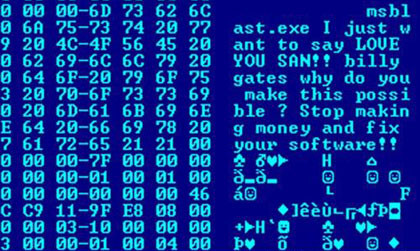
\includegraphics[height=0.5\textheight]{images/Virus_Blaster}
    \end{itemize}
\end{frame}


\end{document}


